\documentclass[nobib]{tufte-book}

% !TeX root = main.tex
% Add the above to each chapter to make compiling the PDF easier in some editors.

\setcounter{secnumdepth}{1}
% \setcounter{tocdepth}{1}

%--------Packages--------
\usepackage{tikz}
\usetikzlibrary{calc, arrows}
\usetikzlibrary{shapes}
\usetikzlibrary{positioning}
\usepackage{booktabs}
\usepackage{tabularx}
\usepackage{longtable}
\usepackage{makecell}
\usepackage{amsmath,amsfonts,amsthm,amssymb,mathrsfs,bbm,mathtools,nicefrac}
\usepackage[shortlabels]{enumitem}
\usepackage{cleveref}
\usepackage[italic]{derivative}
\usepackage{xparse}
\usepackage{upgreek}

%--------Tables--------
\setlength{\LTpre}{0pt}
\setlength{\LTpost}{0pt}

% %--------Literature--------
% \bibliographystyle{plainnat}
% % \usepackage{xargs}
% % \renewcommandx{\cite}[3][1={0pt},2={}]{\sidenote[][#1]{\fullcite[#2]{#3}}}

%--------Graphics/Images--------
\usepackage{graphicx}
% \setkeys{Gin}{width=\linewidth,totalheight=\textheight,keepaspectratio}
\graphicspath{{./figures/}}

% %--------Index--------
\usepackage{imakeidx}
\makeindex[intoc]
\indexsetup{headers={\indexname}{\indexname}}

%--------Theorem Environments--------
\newtheorem{thm}{Theorem}[chapter]
\newtheorem{cor}[thm]{Corollary}
\newtheorem{lem}[thm]{Lemma}

\theoremstyle{definition}
\newtheorem{defn}[thm]{Definition}

\theoremstyle{remark}
\newtheorem{rmk}[thm]{Remark}

\numberwithin{equation}{chapter}

%--------Enumerations--------
\setlist[itemize]{noitemsep,topsep=2pt}

\newlist{thmlist}{enumerate}{1}
\setlist[thmlist]{label=(\alph{thmlisti}), ref=\thethm.(\alph{thmlisti}),noitemsep,topsep=2pt,leftmargin=2\parindent}
\Crefname{thmlisti}{Theorem}{Theorems}

\newlist{corlist}{enumerate}{1}
\setlist[corlist]{label=(\alph{corlisti}), ref=\thethm.(\alph{corlisti}),noitemsep,topsep=2pt,leftmargin=2\parindent}
\Crefname{corlisti}{Corollary}{Corollaries}

\newlist{lemlist}{enumerate}{1}
\setlist[lemlist]{label=(\alph{lemlisti}), ref=\thethm.(\alph{lemlisti}),noitemsep,topsep=2pt,leftmargin=2\parindent}
\Crefname{lemlisti}{Lemma}{Lemmas}

\newlist{nestedlemlist}{enumerate}{1}
\setlist[nestedlemlist]{label=(\roman{nestedlemlisti}), ref=\thethm.(\roman{nestedlemlisti}),noitemsep,topsep=2pt}
\Crefname{nestedlemlisti}{Lemma}{Lemmas}

\newlist{defnlist}{enumerate}{1}
\setlist[defnlist]{label=(\alph{defnlisti}), ref=\thethm.(\alph{defnlisti}),noitemsep,topsep=2pt,leftmargin=2\parindent}
\Crefname{defnlisti}{Definition}{Definitions}

\newlist{rmklist}{enumerate}{1}
\setlist[rmklist]{label=(\alph{rmklisti}), ref=\thethm.(\alph{rmklisti}),noitemsep,topsep=2pt,leftmargin=2\parindent}
\Crefname{rmklisti}{Remark}{Remarks}

%--------Pseudocode--------
\usepackage{xcolor,amsmath}
\usepackage[linesnumbered,ruled,vlined,algochapter]{algorithm2e}
\DontPrintSemicolon
\makeatletter
    \let\c@algocf\c@thm
\makeatother
\crefname{algocf}{alg.}{algs.}
\Crefname{algocf}{Algorithm}{Algorithms}
\SetAlgoSkip{bigskip}

% Define pseudocode formatting
\renewcommand{\KwSty}[1]{\textnormal{\textcolor{blue!90!black}{\ttfamily\bfseries #1}}\unskip}
\renewcommand{\ArgSty}[1]{\textnormal{\ttfamily #1}\unskip}
\SetKwComment{Comment}{\color{green!50!black}// }{}
\renewcommand{\CommentSty}[1]{\textnormal{\ttfamily\color{green!50!black}#1}\unskip}
\newcommand{\assign}{\leftarrow}
\newcommand{\var}{\texttt}
\newcommand{\FuncCall}[2]{\texttt{\bfseries #1(#2)}}
\SetKwProg{Function}{function}{}{}
\renewcommand{\ProgSty}[1]{\texttt{\bfseries #1}}

% %--------Colors-------------
% \definecolor{baby-blue}{cmyk}{0.86,0.33,0.0,0.16,1.0}
\definecolor{blue}{RGB}{02,106,253}
\definecolor{red}{RGB}{245,51,30}
\definecolor{green}{RGB}{96,189,69}
\def\b{\textcolor{blue}}
\def\r{\textcolor{red}}

%--------Colored Theorem-------------
\usepackage[most]{tcolorbox}
\tcbuselibrary{theorems}
\newtcbtheorem
  [use counter*=thm,number within=chapter,crefname={example}{examples},Crefname={Example}{Examples}]%
  {ex}
  {\textbf{Example}}
  {%
%   boxrule=1pt,
%   toprule=1pt,bottomrule=1pt,
    before skip=10pt,after skip=10pt,
    left=0.2cm,right=0.2cm,top=0.2cm,
%   titlerule=0.5em,
%   toptitle=0.1cm,
%   bottomtitle=-0.1cm,
    breakable,
    sharp corners,
    before upper=\setlength{\parskip}{8pt},
    % colback=white,
    % coltitle=black,
    % colframe=blue!100,
    fonttitle=\bfseries,
  }% options
  {ex}% prefix

%--------Margin Tags-------------
\let\marginnote\relax
\usepackage{marginnote}
\NewDocumentCommand{\margintag}{mO{0pt}}{\checkoddpage\ifoddpage{\marginnote{\footnotesize #1}[#2]}\else{\reversemarginpar\marginnote{\footnotesize #1}[#2]}\fi}
\NewDocumentCommand{\marginfootnote}{om}{\footnotemark\margintag{\textsuperscript{\tiny\arabic{footnote}} #2}[#1]}

%--------Equation numbers in text-------------
\makeatletter
\NewDocumentCommand{\embeq}{m}{%
  \leavevmode\hfill\refstepcounter{equation}\textup{\tagform@{\theequation}}\label{#1}%
}
\makeatother

%--------Equation numbers in algorithms-------------
\makeatletter
\NewDocumentCommand{\algeq}{m}{%
  \leavevmode\Comment*[r]{\refstepcounter{equation}\textup{\tagform@{\theequation}}\label{#1}}%
}
\makeatother

\usepackage{etoolbox}
\makeatletter
% Remove right hand margin in algorithm
\patchcmd{\@algocf@start}% <cmd>
  {-1.5em}% <search>
  {0pt}% <replace>
  {}{}% <success><failure>
\makeatother

%--------Allow page breaks in align-------------
\allowdisplaybreaks

% !TeX root = main.tex
% Add the above to each chapter to make compiling the PDF easier in some editors.

% \let\emph\relax
% \DeclareTextFontCommand{\emph}{\bfseries}

\newcommand{\blankpage}{\newpage\hbox{}\thispagestyle{empty}\newpage}
\newcommand{\emptyparagraph}{\paragraph{}\noindent}

\newcommand{\floor}[1]{\left\lfloor #1 \right\rfloor}
\newcommand{\ceil}[1]{\left\lceil #1 \right\rceil}

\newcommand*{\norm}[1]{\| #1 \|}
\newcommand*{\gen}[1]{\langle #1 \rangle}

\newcommand*{\defeq}{\overset{.}{=}}
\newcommand*{\eqdef}{\overset{.}{=}}

\DeclareMathOperator*{\argmax}{arg\,max}
\DeclareMathOperator*{\argmin}{arg\,min}

% \DeclareMathOperator*{\as}{\overset{\mathrm{a.s.}}{=}}

\DeclarePairedDelimiter\parentheses{(}{)}
\DeclarePairedDelimiter\brackets{[}{]}
\DeclarePairedDelimiter\braces{\{}{\}}

\NewDocumentCommand{\inv}{m}{#1^{-1}}

\NewDocumentCommand{\id}{}{\mathrm{id}}

\newcommand{\N}{\mathbb{N}}
\newcommand{\NZ}{\N_0}
\newcommand{\NO}{\N}
\newcommand{\Z}{\mathbb{Z}}
\newcommand{\Q}{\mathbb{Q}}
\newcommand{\R}{\mathbb{R}}
\newcommand{\C}{\mathbb{C}}

\NewDocumentCommand{\woZ}{m}{#1 \setminus \{0\}}

\NewDocumentCommand{\GL}{mm}{\mathrm{GL}_{#1}(#2)}
\NewDocumentCommand{\SL}{mm}{\mathrm{SL}_{#1}(#2)}

% \newcommand{\MLE}{\mathrm{MLE}}
% \newcommand{\MAP}{\mathrm{MAP}}
% \newcommand{\train}{\mathrm{train}}
% \newcommand{\val}{\mathrm{val}}
% \newcommand{\id}{\mathrm{id}}

% \renewcommand{\vec}[1]{\mathbold{#1}}
\newcommand{\mat}[1]{\mathbold{#1}}
% \newcommand{\rvec}[1]{\mathbf{#1}}
% \newcommand{\set}[1]{#1}
% \newcommand{\spa}[1]{\mathcal{#1}}

% \newcommand{\mean}[1]{\overline{#1}}
% \newcommand{\old}[1]{#1^{\mathrm{old}}}

% % common operators
% \NewDocumentCommand{\Ind}{m}{\mathbb{1}\{{#1}\}}
% \NewDocumentCommand{\E}{somo}{\ensuremath{\mathbb{E}\IfValueT{#2}{_{#2}}{} \IfBooleanTF{#1}{#3}{\IfValueTF{#4}{\left[#3\ \middle|\ #4\right]}{\brackets*{#3}}}}}
% \NewDocumentCommand{\Var}{som}{\mathrm{Var}\IfValueT{#2}{_{#2}}{} \IfBooleanTF{#1}{#3}{\brackets*{#3}}}
% \NewDocumentCommand{\Cov}{som}{\mathrm{Cov}\IfValueT{#2}{_{#2}}{} \IfBooleanTF{#1}{#3}{\brackets*{#3}}}
% \NewDocumentCommand{\KL}{mm}{\mathrm{KL}\parentheses*{#1 \| #2}}
% \NewDocumentCommand{\BigO}{m}{\mathcal{O}\parentheses*{#1}}
\NewDocumentCommand{\determ}{m}{\det{\parentheses*{#1}}}
% \NewDocumentCommand{\tr}{m}{\mathrm{tr}\parentheses*{#1}}
% \NewDocumentCommand{\diag}{m}{\mathrm{diag}\parentheses*{#1}}
% \NewDocumentCommand{\pset}{m}{\mathcal{P}\parentheses*{#1}}

% % common vectors, matrices, random vectors, spaces
% \newcommand{\vzero}{\vec{0}}
% \newcommand{\va}{\vec{a}}
% \newcommand{\vap}{\vec{a'}}
% \newcommand{\vas}{\vec{\opt{a}}}
% \newcommand{\vb}{\vec{b}}
% \newcommand{\vf}{\vec{f}}
% \newcommand{\vg}{\vec{g}}
% \newcommand{\vk}{\vec{k}}
% \newcommand{\vr}{\vec{r}}
% \newcommand{\vu}{\vec{u}}
% \newcommand{\vw}{\vec{w}}
% \newcommand{\vx}{\vec{x}}
% \newcommand{\vxp}{\vec{x'}}
% \newcommand{\vxs}{\vec{\opt{x}}}
% \newcommand{\vy}{\vec{y}}
% \newcommand{\vz}{\vec{z}}
% \newcommand{\vepsilon}{\vec{\epsilon}}
% \newcommand{\veta}{\vec{\eta}}
% \newcommand{\vlambda}{\vec{\lambda}}
% \newcommand{\vmu}{\vec{\mu}}
% \newcommand{\vmup}{\vec{\mu'}}
% \newcommand{\vnu}{\vec{\nu}}
% \newcommand{\vomega}{\vec{\omega}}
% \newcommand{\vphi}{\vec{\phi}}
% \newcommand{\vpi}{\vec{\pi}}
% \newcommand{\vvarphi}{\vec{\varphi}}
% \newcommand{\vtheta}{\vec{\theta}}
\newcommand{\mA}{\mat{A}}
% \newcommand{\mC}{\mat{C}}
% \newcommand{\mF}{\mat{F}}
% \newcommand{\mH}{\mat{H}}
\newcommand{\mI}{\mat{I}}
% \newcommand{\mK}{\mat{K}}
% \newcommand{\mL}{\mat{L}}
\newcommand{\mM}{\mat{M}}
% \newcommand{\mQ}{\mat{Q}}
% \newcommand{\mU}{\mat{U}}
% \newcommand{\mW}{\mat{W}}
% \newcommand{\mX}{\mat{X}}
% \newcommand{\mLambda}{\mat{\Lambda}}
% \newcommand{\mSigma}{\mat{\Sigma}}
% \newcommand{\mSigmap}{\mat{\Sigma'}}
% \newcommand{\rQ}{\rvec{Q}}
% \newcommand{\rU}{\rvec{U}}
% \newcommand{\rV}{\rvec{V}}
% \newcommand{\rX}{\rvec{X}}
% \newcommand{\rXp}{\rvec{X'}}
% \newcommand{\rY}{\rvec{Y}}
% \newcommand{\rZ}{\rvec{Z}}
% \newcommand{\sA}{\set{A}}
% \newcommand{\sB}{\set{B}}
% \newcommand{\sC}{\set{C}}
% \newcommand{\sD}{\set{D}}
% \newcommand{\sM}{\set{M}}
% \newcommand{\sS}{\set{S}}
% \newcommand{\sX}{\set{X}}
% \newcommand{\sY}{\set{Y}}
% \newcommand{\spA}{\spa{A}}
% \newcommand{\spB}{\spa{B}}
% \newcommand{\spD}{\spa{D}}
% \newcommand{\spH}{\spa{H}}
% \newcommand{\spP}{\spa{P}}
% \newcommand{\spQ}{\spa{Q}}
% \newcommand{\spX}{\spa{X}}

% \newcommand{\opt}[1]{#1^*}
% \newcommand{\fs}{\opt{f}}
% \newcommand{\ps}{\opt{p}}
% \newcommand{\qs}{\opt{q}}
% \newcommand{\xs}{\opt{x}}
% \newcommand{\ys}{\opt{y}}
% \newcommand{\Bs}{\opt{B}}
% \newcommand{\Qs}{\opt{Q}}
% \newcommand{\hQs}{\opt{\hat{Q}}}
% \newcommand{\Vs}{\opt{V}}
% \newcommand{\pis}{\opt{\pi}}

% % \newcommand{\altpi}{\mbox{\smaller\smaller\smaller$\mathbf{\Pi}$}}
% \newcommand{\altpi}{\vec{\uppi}}

% % distributions
% \NewDocumentCommand{\N}{omm}{\mathcal{N}(\IfValueT{#1}{#1;}{} #2, #3)}
% \NewDocumentCommand{\SN}{o}{\mathcal{N}(\IfValueT{#1}{#1;}{} \vzero, \mI)}
% \NewDocumentCommand{\uSN}{o}{\mathcal{N}(\IfValueT{#1}{#1;}{} 0, 1)}
% \NewDocumentCommand{\GP}{omm}{\mathcal{GP}(\IfValueT{#1}{#1;}{} #2, #3)}
% \NewDocumentCommand{\Unif}{om}{\mathrm{Unif}(\IfValueT{#1}{#1;}{} #2)}
% \NewDocumentCommand{\Bern}{om}{\mathrm{Bern}(\IfValueT{#1}{#1;}{} #2)}
% \NewDocumentCommand{\Bin}{omm}{\mathrm{Bin}(\IfValueT{#1}{#1;}{} #2, #3)}
% \NewDocumentCommand{\Beta}{omm}{\mathrm{Beta}(\IfValueT{#1}{#1;}{} #2, #3)}


\title{Abstract Algebra}
\author{Jonas Hübotter}
\date{Fall 2020}
% \publisher{}
% !TeX root = ../main.tex
% Add the above to each chapter to make compiling the PDF easier in some editors.

\makeatletter
\renewcommand{\maketitlepage}{%
    \cleardoublepage{%
        \begin{fullwidth}%
        \fontsize{12}{12}\selectfont\par\noindent{\@author \\ \noindent \small{Instructor: Frank Himstedt}}%
        \vfill
        \fontsize{40}{46}\selectfont\par\noindent{Abstract Algebra}%
        % \fontsize{14}{16}\selectfont\par\noindent\@date
        \vspace{11.5pc}%
        \vfill
        % \fontsize{14}{16}\selectfont\par\noindent\thanklesspublisher%
        \fontsize{10}{12}\selectfont\par\noindent{\textbf{Contents.} Groups, homomorphisms, cyclic groups, Sylow theorems, and solvable groups. Rings, ideals, polynomial rings, irreducibility of polynomials. Fields, field extensions, Galois theory, solvable polynomials.} \\[5pt]
        \fontsize{10}{12}\selectfont\par\noindent{Contributions are welcome at \url{https://github.com/jonhue/algebra}.}
        \end{fullwidth}%
    }%
    \thispagestyle{empty}%
    \clearpage
}
\makeatother


\usepackage{letltxmacro}
\begin{document}
    \frontmatter

    \maketitle

    % !TeX root = ../main.tex
% Add the above to each chapter to make compiling the PDF easier in some editors.

\begin{fullwidth}
\thispagestyle{empty}
\setlength{\parindent}{0pt}

\null\vfill

\section*{\smallcaps{Acknowledgement}}
The contents of this summary are based on the ``Algebra'' lecture given by \mbox{Frank Himstedt} at the Technical University of Munich in fall of 2020.

% \makeatletter
% \par\noindent\@title
% \selectfont\par\noindent\@author
% \selectfont\par\noindent\@date
% \makeatother

\end{fullwidth}


    \tableofcontents

    \mainmatter

	\part{Groups}\label{cha:groups}
    % !TeX root = ../main.tex
% Add the above to each chapter to make compiling the PDF easier in some editors.

\chapter{Groups and Homomorphisms}
\section{Groups}
\begin{defn}[Semigroup, Monoid, and Group]\leavevmode
\begin{defnlist}
    \item A set $G$ with a mapping $\cdot$ on $G$ (that is, $\cdot: G \times G \to G$) is named \begin{itemize}
        \item \emph{semigroup}\index{semigroup} if $\forall a, b, c \in G.\ (a \cdot b) \cdot c = a \cdot (b \cdot c)$; \margintag{\emph{associativity}\index{associativity}}
        \item \mbox{\emph{monoid}\index{monoid} if it is a semigroup and $\exists e \in G.\ \forall a \in G.\ e \cdot a = a \cdot e = a$; \margintag{$e$ is called \emph{neutral element}\index{neutral element}}}
        \item \emph{group}\index{group} if it is a monoid and $\forall a \in G.\ \exists a' \in G.\ a \cdot a' = a' \cdot a = e$. \margintag{$a'$ is the \emph{inverse element}\index{inverse element} of $a$}
    \end{itemize}
    
    \item A group $(G,\cdot)$ is named \emph{abelian}\index{abelian group} or \emph{commutative}\index{commutativity} if the group operation $\cdot$ is commutative under elements of $G$, \begin{align}
        \forall a, b \in G.\quad a \cdot b = b \cdot a.
    \end{align}
    
    \begin{marginfigure}
        We denote groups by $(G,\cdot)$. If the group operation $\cdot$ is clear from context, we refer to the group simply as $G$. Subsequently, we also write $a b$ instead of $a \cdot b$.
    \end{marginfigure}
\end{defnlist}
\end{defn}

\begin{rmk}
Let $G$ be a group. Then, \begin{rmklist}
    \item there is exactly one neutral element $e \in G$ and for every $a \in G$ there is exactly one inverse element $a' \in G$, which we call $\inv{a}$;
    \item the mapping on $G$, which we refer to by $\cdot$, may be resembled by any symbol;
    \item if $G$ is abelian, often \begin{itemize}
        \item $+$ is used instead of $\cdot$,
        \item $0$ is used instead of $e$, and
        \item $-a$ is used instead of $\inv{a}$.
    \end{itemize}
\end{rmklist}
\end{rmk}

\begin{ex}{Semigroups, monoids, and groups}{}
\begin{center}
\setlength\tabcolsep{5pt}
\begin{tabular}{lrrrrr}
\toprule
 & $(\NO,+)$ & $(\NZ,+)$ & $(\Z,+)$ & $(\Z,\cdot)$ & $(\woZ{\Q},\cdot)$ \\
 \midrule
 semigroup & yes & yes & yes & yes & yes \\
 \addlinespace
 monoid & no & yes & yes & yes & yes \\
 \addlinespace
 group & yes & no & yes & no & yes \\
 \bottomrule
\end{tabular}
\end{center}
\end{ex}

\begin{ex}{General linear and special linear group}{}
The \emph{general linear group}\index{general linear group} $\GL{n}{K}$ is the group of invertible\marginfootnote{Recall from linear algebra that a matrix $\mA$ is invertible iff $\det{\mA} \neq 0$.} ${n \times n}$ linear maps over a field\marginfootnote[1\baselineskip]{A \emph{field}\index{field} is a set of elements with well-defined operations for addition, subtraction, multiplication, and division. We give a formal definition in \cref{defn:field}. Examples of fields are the rational numbers $\Q$, the real numbers $\R$, and the complex numbers $\C$.} $K$, \begin{align}
    \GL{n}{K} \defeq \{\mA \in K^{n \times n} \mid \det{\mA} \neq 0\}.
\end{align}

The \emph{special linear group}\index{special linear group} $\SL{n}{K}$ is the group of normed linear maps over the field $K$, \begin{align}
    \SL{n}{K} \defeq \{\mA \in K^{n \times n} \mid \det{\mA} = 1\}.
\end{align}

The group operation of $\GL{n}{K}$ and $\SL{n}{K}$ is matrix multiplication. Their neutral element is the identity matrix $\mI$, and the inverse elements are the matrix inverses $\inv{\mA}$.
\end{ex}

\begin{ex}{Abelian groups}{}
\begin{itemize}
    \item $(\Z,+)$
    \item $(\Q,+)$
    \item $(\R,+)$
    \item $(\woZ{\R},\cdot)$
\end{itemize}
\end{ex}

\begin{ex}{Symmetric group}{}
The \emph{symmetric group}\index{symmetric group} $S_n$ is the group of bijections on the set $[n]$, \begin{align}
    S_n \defeq \{\sigma : [n] \to [n] \mid \text{$\sigma$ is bijective}\},
\end{align} with the function composition ``$\circ$'' as mapping.

Elements of the symmetric group ${\sigma \in S_n}$ are called \emph{permutations}\index{permutation}. The neutral element of the symmetric group is the identity $\id$, which maps each input to itself.

There are multiple ways of representing permutations. Perhaps the most natural representation of ${\sigma \in S_n}$ is a mapping in \emph{two-line notation}\index{two-line notation}, \begin{align}
    \sigma = \begin{pmatrix}
        1 & 2 & \cdots & n \\
        \sigma(1) & \sigma(2) & \cdots & \sigma(n) \\
    \end{pmatrix},
\end{align} or in \emph{one-line notation}\index{one-line notation} by simply omitting the first line, \begin{align}
    \sigma = (\sigma(1)\ \sigma(2)\ \cdots\ \sigma(n)).
\end{align}

An alternative characterization of a permutation is as a product of (disjoint) cycles. A \emph{cycle}\index{cycle} ${\rho \in S_n}$ is a permutation that maps a subset of numbers ${\{i_1, i_2, \dots, i_r\} \subseteq [n]}$ in a cyclic fashion. That is, \begin{align}
    \rho(i_1) = i_2,\quad \rho(i_2) = i_3,\quad \cdots\quad \rho(i_{r-1}) = i_r,\quad \rho(i_r) = i_1,
\end{align} leaving all other ${j \in [n]}$ fixed. We denote such a cycle by \begin{align}
    \rho = (i_1\ i_2\ \cdots\ i_r).
\end{align} A cycle of length $r$, is also called \emph{$r$-cycle}. 2-cycles are called \emph{transpositions}\index{transposition}.

Every permutation ${\sigma \in S_n}$ can be written as a ``product'' (i.e., composition), \begin{align}
    \sigma = \rho_1 \cdots \rho_s,
\end{align} where $\rho_i$ are cycles with pairwise disjunct elements. This is also known as the \emph{cycle notation}\index{cycle notation} of $\sigma$. Note that the ordering of $\rho_1, \dots \rho_s$ does not matter, as their elements are disjoint.

The cycle lengths $r_1, \dots, r_s$ (in descending order) of $\rho_1, \dots, \rho_s$ are the \emph{cycle type}\index{cycle type} of $\sigma$.

\begin{rmk}
The symmetric group is not abelian.
\end{rmk}\vspace{-20pt}\begin{proof}
We have $(1\ 2)(2\ 3) = (2\ 3\ 1)$ and $(2\ 3)(1\ 2) = (1\ 3\ 2)$.
\end{proof}
\end{ex}

\begin{lem}[Notation and Rules]
Let $(G,\cdot)$ be a group. \begin{lemlist}
    \item For $a \in G, n \in \NZ$, we write \begin{itemize}
        \item $a^n \defeq \underbrace{a \cdot a \cdots a}_{\text{$n$ many}}$,
        \item $a^0 \defeq e$, and
        \item $a^{-n} \defeq \underbrace{\inv{a} \cdot \inv{a} \cdots \inv{a}}_{\text{$n$ many}}$.
    \end{itemize}
    
    \item $\forall a, b \in G.\ \forall m, n \in \Z.$ \begin{nestedlemlist}
        \item $\inv{(\inv{a})} = a$
        \item $a^m \cdot a^n = a^{m+n}$, $(a^m)^n = a^{m \cdot n}$
        \item $\inv{(a \cdot b)} = \inv{b} \cdot \inv{a}$
    \end{nestedlemlist}
\end{lemlist}
\end{lem}
\begin{proof}[Proof of (b)(iii)] $(a \cdot b) \cdot \inv{b} \cdot \inv{a} = a \cdot \underbrace{(b \cdot \inv{b})}_{=e} \cdot \inv{a} = a \cdot \inv{a} = e$.
\end{proof}

\begin{defn}[Subgroup]\label{defn:subgroup}
A subset $U \subseteq G$ is called a \emph{subgroup}\index{subgroup} of a group $G$ (denoted $U \subgroup G$) if $U$ itself is a group with mapping $\cdot$. That is, $U$ is a subgroup iff \begin{defnlist}
    \item $e \in U$; \margintag{$U$ contains the neutral element}
    \item $\forall a, b \in U.\quad a \cdot b \in U$; and \margintag{the mapping $\cdot$ is closed wrt. $U$}
    \item $\forall a \in U.\quad \inv{a} \in U.$ \margintag{the mapping $\inv{(\dots)}$ is closed wrt. $U$}
\end{defnlist} Associativity follows from $G$ being a group.
\end{defn}

\begin{ex}{Subgroups}{}
\begin{itemize}
    \item $\{e\}, G \subgroup G$ (\emph{trivial subgroups}\index{trivial subgroups})
    \item $\SL{n}{K} \subgroup \GL{n}{K}$
    \item Let $2\Z \defeq \{2m \mid m \in \Z\}$, then $(2\Z,+) \subgroup (\Z,+)$
\end{itemize}
\end{ex}

\begin{rmk}\label{rmk:cap_subgroup}
If $\{U_i\}_{i \in I}$ are subgroups of $G$, then $\bigcap_{i \in I} U_i \subgroup G$.
\end{rmk}

\begin{defn}[Generated Subgroup]
For any $M \subseteq G$, \begin{align}
    \gen{M} \defeq \bigcap_{\substack{U \subgroup G \\ M \subseteq U}} U \subgroup G, \margintag{by \cref{rmk:cap_subgroup}}
\end{align} is the \emph{subgroup generated by $M$}\index{generated subgroup}. In particular, $\gen{M}$ is the ``smallest'' subgroup that includes $M$.
\end{defn}

\begin{lem}
For $M \neq \emptyset$, we have \begin{align}
    \gen{M} = \{a_1 \cdot a_2 \cdots a_n \mid n \in \N, \text{$a_i \in M$ or $\inv{a_i} \in M$}\}.
\end{align}
\end{lem} \begin{proof}[Proof (sketch)]\leavevmode
Let $N \defeq \{a_1 \cdot a_2 \cdots a_n \mid n \in \N, \text{$a_i \in M$ or $\inv{a_i} \in M$}\}$.
\begin{itemize}
    \item \underline{$\gen{M} \subseteq N$}: $N \subgroup G$ and $M \subseteq N \implies \gen{M} \subseteq N$ \margintag{using that $\gen{M}$ is the smallest subgroup including $M$}
    \item \underline{$N \subseteq \gen{M}$}: if $U \subgroup G$ with $M \subseteq U$, then $U$ includes all of these products $\implies N \subseteq U \implies N \subseteq \gen{M}$ \qedhere
\end{itemize}
\end{proof}

\begin{ex}{Generated subgroup}{}
$S_3 = \{\id, \underbrace{(1\ 2)}_{\tau_1}, \underbrace{(1\ 3)}_{\tau_2}, \underbrace{(2\ 3)}_{\tau_3}, \underbrace{(1\ 2\ 3)}_{\sigma_1}, \underbrace{(1\ 3\ 2)}_{\sigma_2}\} = \gen{\{\underbrace{(1\ 2)}_{\tau_1}, \underbrace{(1\ 2\ 3)}_{\sigma_1}\}}$.
\end{ex}

\begin{defn}[Cyclic Group]
A group $G$ is \emph{cyclic}\index{cyclic group} if $\exists a \in G$ with \begin{align}
    G = \gen{a} \defeq \gen{\{a\}} = \{a^m \mid m \in \Z\}.
\end{align} Such an $a \in G$, is called a \emph{generator}\index{generator} of $G$.
\end{defn}

\begin{marginfigure}
    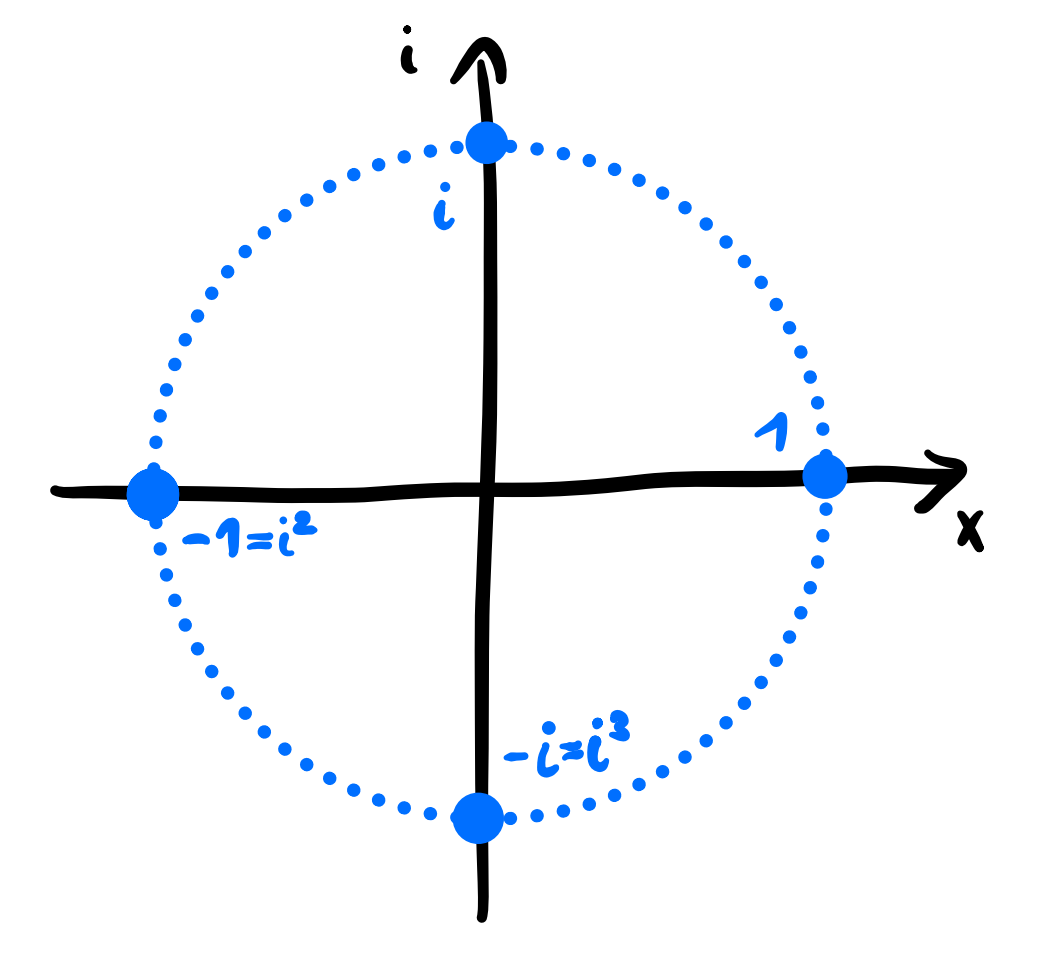
\includegraphics[width=\textwidth]{c_cyclic_subgroup.png}
    \caption{An illustration of the cyclic subgroup $\gen{i}$ in the complex plane.}
\end{marginfigure}

\begin{ex}{Cyclic groups}{}
\begin{itemize}
    \item $\gen{i} = \{i^m \mid m \in \Z\}$ is a cyclic subgroup of $(\woZ{\C},\cdot)$, \begin{align*}
        \gen{i} &= \{\dots, \underbrace{i^{-2}}_{=-1}, \underbrace{i^{-1}}_{=-i}, 1, i, \underbrace{i^2}_{=-1}, \underbrace{i^3}_{=-i}, \underbrace{i^4}_{=1}, \underbrace{i^5}_{=i}, \dots\} \\
                &= \{1, i, -1, -i\}.
    \end{align*}
    \item $(\Z,+) = \gen{1} = \{\dots, -2, -1, 0, 1, 2, \dots\}$ is cyclic
\end{itemize}
\end{ex}

\begin{defn}[Order]\index{order}
Let $G$ be a group.
\begin{defnlist}
    \item The cardinality $|G| \in \wInfty{\N}$ is called \emph{order} of the group $G$.
    \item For any $a \in G$, $o(a) \defeq |\gen{a}|$ is the \emph{order} of the element $a$.
\end{defnlist} If $|G| < \infty$, $G$ is called \emph{finite}\index{finite group}.
\end{defn}

\begin{lem}
If $k \defeq o(a) < \infty$, we have \begin{lemlist}
    \item $o(a) = \min\{j \in \N \mid a^j = e\}$;
    \item $\gen{a} = \{e, a, a^2, \dots, a^{k-1}\}$; and
    \item\label{lem:order_identity} For any $j \in \Z$, $a^j = e \iff \divides{o(a)}{j}$.\footnote{We use $\divides{a}{b}$ to denote that $a$ divides $b$.}
\end{lemlist}
\end{lem} \begin{proof}
We write $m \defeq \min\{j \in \N \mid a^j = e\}$. \begin{itemize}
    \item \underline{$\{e, a, a^2, \dots, a^{m-1}\} \subseteq \gen{a}$}: Let us fix an arbitrary $j \in \N$. We have, \begin{align*}
        o(a) = |\gen{a}| < \infty &\implies \exists j' > j.\ a^j = a^{j'} \margintag{as the order of $a$ is finite} \\
                                  &\implies a^{j'-j} = e \margintag{by multiplying from the right with $a^{-j}$} \\
                                  &\implies \text{$m$ exists and $\{e, a, a^2, \dots, a^{m-1}\} \subseteq \gen{a}$}. \margintag{as $j'-j \in \N$ is again a natural number}
    \end{align*}
    \item \underline{$\gen{a} \subseteq \{e, a, a^2, \dots, a^{m-1}\}$}: We fix any $n \in \Z$. Then, by \emph{long division}\index{long division}, there exist $q, r \in \Z$ and $0 \leq r < m$ with $n = q \cdot m + r$. This yields, \begin{align*}
        a^n = a^{q \cdot m + r} = \underbrace{(a^m)^q}_{=e} \cdot a^r = a^r \in \{e, a, a^2, \dots, a^{m-1}\}.
    \end{align*}
\end{itemize} This proves that $m = o(a)$ and $\gen{a} = \{e, a, a^2, \dots, a^{m-1}\}$. It also follows that \begin{align*}
    a^n = e \iff r = 0 \iff \divides{m}{n}. &\qedhere
\end{align*}
\end{proof}

\begin{rmk}
For a finite cyclic group $\gen{a} = \{e, a, a^2, \dots, a^{k-1}\}$ of order $k$, we have $a^{k-j} = a^{-j}$.
\end{rmk}

\begin{ex}{Order}{}
\begin{itemize}
    \item Let us consider $\GL{2}{\R}$. Then, \begin{align*}
        \mA = \begin{bmatrix}
            2 & 0 \\
            0 & 2 \\
        \end{bmatrix} &\implies \forall n \in N.\ \mA^n = \begin{bmatrix}
            2^n & 0 \\
            0 & 2^n \\
        \end{bmatrix} \neq \mI \\ &\implies o(\mA) = \infty, \\
        \mB = \begin{bmatrix}
            0 & 1 \\
            -1 & 0 \\
        \end{bmatrix} &\implies \begin{multlined}[t]\mB^2 = \begin{bmatrix}
            -1 & 0 \\
            0 & -1 \\
        \end{bmatrix}, \\ \mB^3 = -\mB = \begin{bmatrix}
            0 & -1 \\
            1 & 0 \\
        \end{bmatrix}, \mB^4 = (\mB^2)^2 = \mI\end{multlined} \\ &\implies o(\mB) = 4.
    \end{align*}
    
    \item $|S_n| = |\{\sigma : [n] \to [n] \mid \text{$\sigma$ is bijective}\}| = n!$
\end{itemize}
\end{ex}

\begin{ex}{Subgroups of $S_3$}{s3_subgroups}
Let us find the subgroups of \begin{align*}
    S_3 = \{\id, (1\ 2), (1\ 3), (2\ 3), (1\ 2\ 3), (1\ 3\ 2)\}.
\end{align*} We immediately obtain the trivial subgroups $\{\id\}$ and $S_3$ or order $1$ and $6$, respectively. It is a simple exercise to confirm the following cyclic subgroups: \begin{itemize}
    \item $\gen{(1\ 2)} = \{\id, (1\ 2)\}$
    \item $\gen{(1\ 3)} = \{\id, (1\ 3)\}$
    \item $\gen{(2\ 3)} = \{\id, (2\ 3)\}$
    \item $\gen{(1\ 2\ 3)} = \gen{(1\ 3\ 2)} = \{\id, (1\ 2\ 3), (1\ 3\ 2)\}$
\end{itemize} The first three subgroups generated by 2-cycles are of order 2, the last subgroup generated by the 3-cycles is of order 3.

Observe that the subgroup orders are divisors of the group order. This is not coincidental, we will make this precise in the following. In doing so, we will also find that our list of subgroups of $S_3$ was indeed exhaustive.
\end{ex}

\begin{marginfigure}
    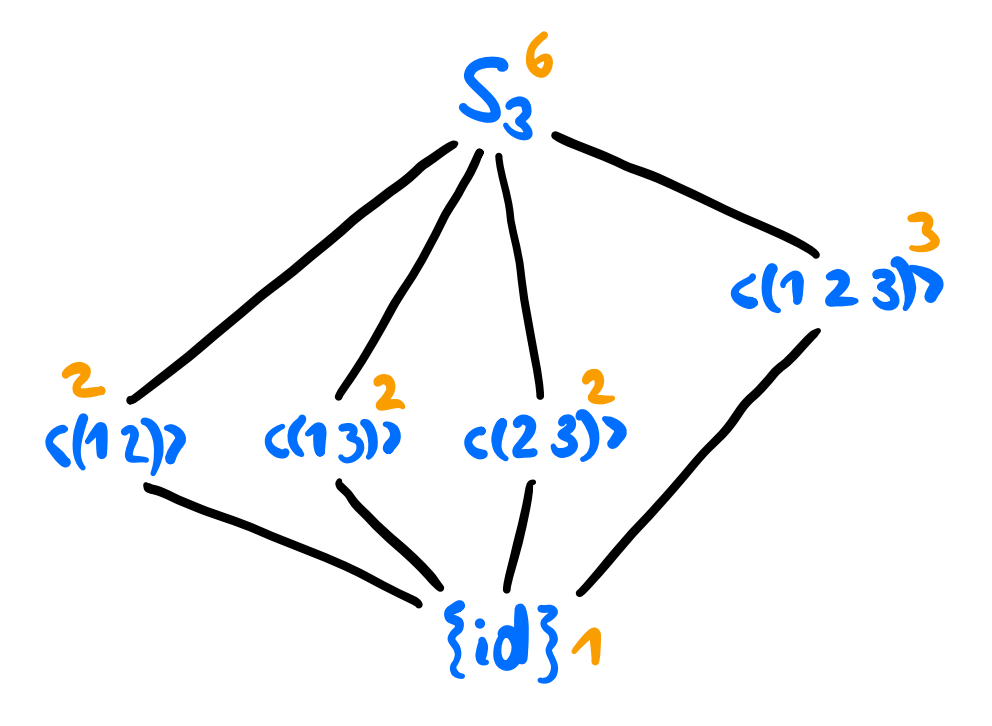
\includegraphics[width=\textwidth]{s3_subgroup_graph.png}
    \caption{Subgroup graph of the symmetric group $S_3$. The order of the subgroups is shown in orange.}\label{fig:s3_subgroup_graph}
\end{marginfigure}
    
The subgroup structure of a group $G$ can be graphically represented in a \emph{subgroup graph}\index{subgroup graph}. Subgroups of $G$ are represented as vertices. Groups $U$ and $V$ are connected if $U \subgroup V$ and there exists no subgroup ``between'' $U$ and $V$. An example is given in \cref{fig:s3_subgroup_graph}.

\begin{defn}[Cosets and Index]
Let $U \subgroup G$ be a subgroup.
\begin{defnlist}
    \item For $a \in G$, \begin{align}
        aU &\defeq \{a \cdot u \mid u \in U\}, \label{eq:left_coset} \\
        Ua &\defeq \{u \cdot a \mid u \in U\},
    \end{align} are the left\index{left coset} and right\index{right coset} \emph{coset}\index{coset} of $U$ in $G$, respectively.
    \item\label{defn:index} The \emph{index}\index{index} $[G : U] \defeq |\{aU \mid a \in G\}|$ of $U$ in $G$ is defined as the number of cosets of $U$ in $G$.\footnote{The number of left cosets is identical to the number of right cosets.}
\end{defnlist}
\end{defn}

\begin{lem}
For all $a, b \in G$, we have
\begin{lemlist}
    \item $aU = U \iff a \in U$
    \item\label{lem:cosets_eq} $aU = bU \iff \inv{a} b \in U$
    \item $aU \cap bU \neq \emptyset \iff aU = bU$
    \item $G = \bigcup_{a \in G} aU$
    \item\label{lem:cosets_size} $|aU| = |U|$
\end{lemlist}
\end{lem} \begin{proof}[Proof of (e)]
$U \to aU, u \mapsto a \cdot u$ is a bijective mapping. Hence, domain and codomain are of the same size.
\end{proof}

\begin{thm}[Lagrange's Theorem]\index{Lagrange's theorem}\label{thm:lagrange}
If $G$ is a finite group and $U \subgroup G$ is some subgroup, then \begin{align}
    |G| = |U| \cdot [G : U].
\end{align} In particular, $|U|$ and $[G : U]$ are divisors of $|G|$.
\end{thm} \begin{proof}
Let $r \defeq \Index{G}{U}$. Then we can write $G$ as a disjoint union of cosets, \begin{align*}
    G = a_1 U \cupdot a_2 U \cupdot \cdots \cupdot a_r U.
\end{align*} We have, \begin{align*}
    |G| = \sum_{i=1}^r |a_i U| = r \cdot |U| = \Index{G}{U} \cdot |U|. \margintag{using that $|a_i U| = |U|$ by \cref{lem:cosets_size}} &\qedhere
\end{align*}
\end{proof}

\begin{cor}
Let $G$ be a finite group. Then we have for any $a \in G$, \begin{corlist}
    \item $\divides{o(a)}{|G|}$
    \item $a^{|G|} = e$ \quad (\emph{Fermat's little theorem}\index{Fermat's little theorem})
\end{corlist}
\end{cor} \begin{proof}
\leavevmode\begin{corlist}
\item By \hyperref[thm:lagrange]{Lagrange's theorem}, $\divides{|\gen{a}|}{|G|}$.
\item By \cref{lem:order_identity}, $a^{|G|} = e \iff \divides{o(a)}{|G|}$. \qedhere
\end{corlist}
\end{proof}

\begin{cor}\label{cor:prime_group_is_cyclic}
Let $G$ be a group such that $|G| = p$ where $p$ is prime. Then, $G$ is cyclic.
\end{cor} \begin{proof}
\begin{align*}
    |G| > 1 &\implies \exists a \in G \setminus \{e\} \\
            &\implies \divides{1 \neq |\gen{a}|}{|G|} \margintag{using that $o(a) \geq 2$ if $a \neq e$ and \hyperref[thm:lagrange]{Lagrange's theorem}} \\[5pt]
            &\implies |\gen{a}| = p = |G|. \margintag{using that $|G|$ only has divisors $1$ and $p$}
\end{align*} Therefore, $\gen{a} = G$.
\end{proof}

\begin{ex}{Subgroups of $S_3$ (continued)}{}
We will now see that $S_3$ has exactly four non-trivial subgroups, proving that we have found all subgroups of $S_3$ in \cref{ex:s3_subgroups}.

Let ${U \subgroup S_3}$ be a non-trivial subgroup. By \hyperref[thm:lagrange]{Lagrange's theorem}, we have ${\divides{|U|}{|S_3| = 3! = 6}}$. As we have excluded the trivial subgroups $\{\id\}$ and $S_3$, we know that ${|U| \neq 1, 6}$. This leaves us with ${|U| \in \{2,3\}}$.

Observe that $2$ and $3$ are prime, hence, by \cref{cor:prime_group_is_cyclic} $U$ must be cyclic. Recall that we have already enumerated all (four) cyclic subgroups of $S_3$ in \cref{ex:s3_subgroups}.
\end{ex}

\section{Homomorphisms}
We will now consider two groups $(G,\cdot)$ and $(H,\cdot)$. To understand the relationship between $G$ and $H$, it is useful to look at mappings between the two groups. A special mapping that (as we will see) preserves the structure of a group, is the group homomorphism.

\begin{defn}[(Group) Homomorphism]
\leavevmode\begin{defnlist}
    \item The mapping $\varphi : G \to H$ is called a \emph{(group) homomorphism}\index{homomorphism}\index{group homomorphism} if \begin{align}
        \forall a, b \in G.\quad \varphi(a \cdot b) = \varphi(a) \cdot \varphi(b). \label{eq:homomorphism}
    \end{align} The homomorphism $\psi : G \to G$ is called \emph{endomorphism}\index{endomorphism} of $G$.
    \item The set of elements that are mapped to the neutral element $e_H$, \begin{align}
        \ker{\varphi} \defeq \{a \in G \mid \varphi(a) = e_H\} \subseteq G, \label{eq:kernel}
    \end{align} is called the \emph{kernel}\index{kernel} of $\varphi$.
    \item The set of elements in the codomain $H$ that $\varphi$ maps to, \begin{align}
        \im{\varphi} \defeq \{\varphi(a) \mid a \in G\} \subseteq H,
    \end{align} is called the \emph{image}\index{image} of $\varphi$.
\end{defnlist}
\end{defn}

\begin{ex}{Homomorphisms}{homomorphisms}
\begin{itemize}
    \item ${\varphi : G \to H, a \mapsto e_H}$ is the \emph{trivial homomorphism}\index{trivial homomorphism}
    
    \item For any field $K$, ${\det : \GL{n}{K} \to \woZ{K}, \mA \mapsto \det{\mA}}$ is a homomorphism due to the multiplicativity of the determinant.\marginfootnote{Recall that $\det{(\mA \cdot \mB)} = \det{\mA} \cdot \det{\mB}$.} We have for its kernel, \begin{align}
        \ker{\det} = \{\mA \in \GL{n}{K} \mid \det{\mA} = 1\} = \SL{n}{K}. \label{eq:det_kernel}
    \end{align}
    
    \item Let us consider the \emph{sign}\index{sign} of a permutation, \begin{align}
        \sgn : S_n \to \{-1, 1\}, \sigma \mapsto (-1)^{N(\sigma)},
    \end{align} where $N(\sigma)$ is the number of inversions in $\sigma$. An \emph{inversion}\index{inversion} in $\sigma$ is a pair of elements that is out of order. More formally, \begin{align}
        N(\sigma) = |\{(i,j) \mid \text{$i < j$ and $\sigma(i) > \sigma(j)$}\}|.
    \end{align} For an $r$-cycle the sign reduces to, \begin{align}
        \sgn{\underbrace{(i_1\ \cdots\ i_r)}_{\text{$r$-cycle}}} = (-1)^{r-1}.
    \end{align}
    
    It can be shown that $\sgn$ is a homomorphism, that is, \begin{align}
        \forall \sigma, \tau \in S_n.\quad \sgn{(\sigma \circ \tau)} = \sgn{\sigma} \cdot \sgn{\tau}.
    \end{align} The kernel of $\sgn$ is the set of permutations with positive sign, \begin{align}
        \ker{\sgn} = \{\sigma \in S_n \mid \sgn{\sigma} = 1\} \eqdef A_n. \label{eq:alternating_group}
    \end{align} This set forms again a group, which is known as the \emph{alternating group}\index{alternating group} $A_n$.
    
    \item Within the group $(\Z,+)$, $\varphi : \Z \to \Z, m \mapsto 2 m$ is an endomorphism.
\end{itemize}
\end{ex}

\begin{lem}[Properties of Homomorphisms]
Let $\varphi : G \to H$ be a homomorphism. Then,
\begin{lemlist}
    \item $\varphi(e_G) = e_H$
    \item $\forall g \in G.\ \varphi(\inv{g}) = \inv{\varphi(g)}$
    \item\label{lem:homomorphism_kernel_subgroup} $\ker{\varphi} \subgroup G$ and $\im{\varphi} \subgroup H$
    \item $\text{$\varphi$ injective} \iff \ker{\varphi} = \{e_G\}$
    \item if $\psi : H \to K$ is a homomorphism, then $\psi \circ \varphi : G \to K$ is a homomorphism
\end{lemlist}
\end{lem} \begin{marginfigure}
    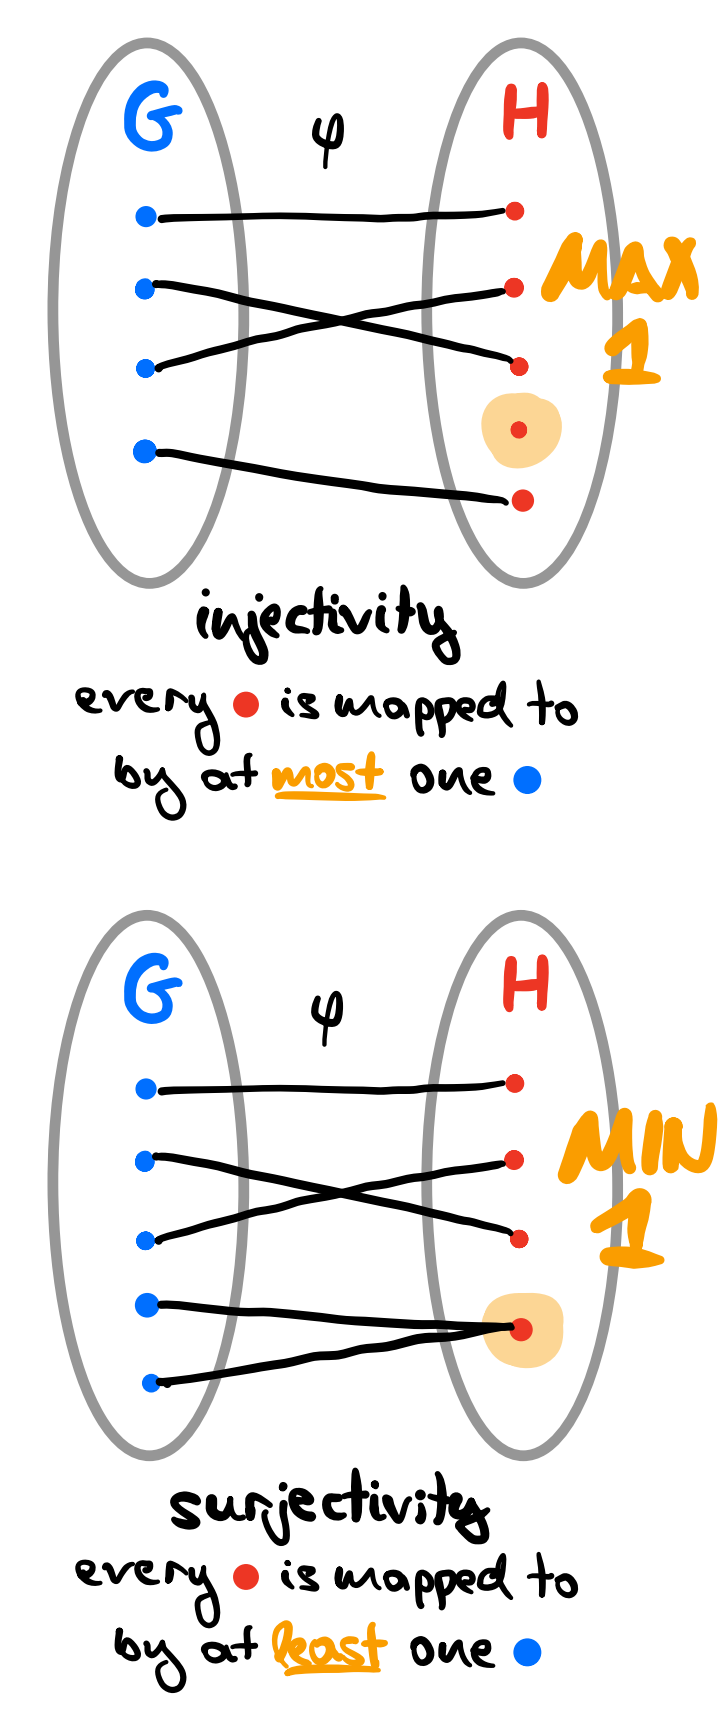
\includegraphics[width=\textwidth]{injective_surjective.png}
    \caption{An illustration of \emph{injectivity}\index{injective} and \emph{surjectivity}\index{surjective}. When a function $\varphi$ is injective, $\varphi(a) = \varphi(b)$ implies $a = b$. We call a function \emph{bijective}\index{bijective} is it is both injective and surjective, i.e., a one-to-one mapping.}
\end{marginfigure} \begin{proof}
\leavevmode\begin{lemlist}
    \item We have $\varphi(e_G) = \varphi(e_G \cdot e_G) = \varphi(e_G) \cdot \varphi(e_G)$, using the compatibility of a homomorphism with the group structure \eqref{eq:homomorphism}. By multiplying with $\inv{\varphi(e_G)}$ from one side, we obtain that this statement is true if and only if $\varphi(e_G) = e_H$.
    
    \item Again, using the homomorphism property, we have, \begin{align*}
        e_H = \varphi(e_G) = \varphi(g \cdot \inv{g}) = \varphi(g) \cdot \varphi(\inv{g}).
    \end{align*} By multiplying from the left with $\inv{\varphi(g)}$, we obtain that this statement is true if and only if $\inv{\varphi(g)} = \varphi(\inv{g})$.
    
    \item Let us confirm the properties of subgroups for $\ker{\varphi} \subgroup G$. The proof is analogous for $\im{\varphi} \subgroup H$. By \cref{defn:subgroup}, we need to show, \begin{nestedlemlist}
        \item $e_G \in \ker{\varphi}$ follows immediately from (a)
        \item $\forall a, b \in \ker{\varphi}.\ \varphi(a \cdot b) = \varphi(a) \cdot \varphi(b) = e_H \cdot e_H = e_H$. Therefore, $\ker{\varphi}$ is closed under the group operation, $a \cdot b \in \ker{\varphi}$.
        \item $\forall a \in \ker{\varphi}.\ \varphi(\inv{a}) = \inv{\varphi(a)} = \inv{e_H} = e_H$. Therefore, $\ker{\varphi}$ is closed under inversion, $\inv{a} \in \ker{\varphi}$.
    \end{nestedlemlist}
    $\implies \ker{\varphi} \subgroup G$.
    
    \item \begin{itemize}
        \item \underline{``$\Rightarrow$''}: Let $\varphi$ be injective. We want to show that $\ker{\varphi} = \{e_G\}$. Note that (a) already implies $\{e_G\} \subseteq \ker{\varphi}$. To show $\ker{\varphi} \subseteq \{e_G\}$, let $a \in \ker{\varphi}$. Then, \begin{align*}
            \varphi(a) = e_H \overset{(a)}{=} \varphi(e_H).
        \end{align*} As $\varphi$ is injective, it follows that $a = e_H$.
        \item \underline{``$\Leftarrow$''}: Let $\ker{\varphi} = \{e_G\}$. We want to show that $\varphi$ is injective. Let $a, b \in G$ with $\varphi(a) = \varphi(b)$. By multiplying from the right with $\inv{\varphi(b)}$, we obtain, \begin{align*}
            e_H = \varphi(a) \cdot \inv{\varphi(b)} = \varphi(a) \cdot \varphi(\inv{b}) = \varphi(a \cdot \inv{b}).
        \end{align*} As the kernel of $\varphi$ only contains $e_G$, we follow, \begin{align*}
            e_G = a \cdot \inv{b} \overset{\cdot b}{\implies} a = b \implies \text{$\varphi$ injective}.
        \end{align*}
    \end{itemize}
    
    \item Let $a, b \in G$. Then, \begin{align*}
        (\psi \circ \varphi)(a \cdot b) &= \psi(\varphi(a \cdot b)) = \psi(\varphi(a) \cdot \varphi(b)) \margintag{using that $\varphi$ is a homomorphism} \\
        &= \psi(\varphi(a)) \cdot \psi(\varphi(b)) = (\psi \circ \varphi)(a) \cdot (\psi \circ \varphi)(b). \margintag{using that $\psi$ is a homomorphism} \qedhere
    \end{align*}
\end{lemlist}
\end{proof}

\begin{defn}[Isomorphism]
\leavevmode\begin{defnlist}
    \item The mapping $\varphi : G \to H$ is called an \emph{isomorphism}\index{isomorphism} if $\varphi$ is a homomorphism and bijective. The isomorphism $\psi : G \to G$ is called an \emph{automorphism}\index{automorphism} of $G$.
    \item $G$ and $H$ are called \emph{isomorphic} (denoted $G \isom H$) if there exists an isomorphism $\varphi : G \to H$.
    \item $\Aut{G} \defeq \{\psi : G \to G \mid \text{$\psi$ automorphism}\}$ forms a group under function composition ``$\circ$''. This group is called the \emph{automorphic group}\index{automorphic group} of $G$.
\end{defnlist}
\end{defn}

\begin{rmk}
If $\varphi : G \to H$ is an isomorphism, then $\inv{\varphi} : H \to G$ is an isomorphism.
\end{rmk}

\begin{ex}{Isomorphisms}{}
\begin{itemize}
    \item Given a group $G$ and an arbitrary element $g \in G$, \begin{align}
        i_g : G \to G, x \mapsto g \cdot x \cdot \inv{g},
    \end{align} is the \emph{inner automorphism}\index{inner automorphism} of the so-called \emph{conjugating element}\index{conjugating element} $g$. This isomorphism corresponds to the conjugation group action (also called \emph{(left) conjugation}\index{conjugation} by $g$), which we will encounter again in \cref{sec:groups:actions}.
    
    \item $\exp : (\R,+) \to (\RgZ,\cdot), x \mapsto e^x$ is an isomorphism.\marginfootnote{$\exp$ is a homomorphism due to $e^{x+y} = e^x e^y$. As $\exp$ is strictly monotonically increasing, it is bijective.}
\end{itemize}
\end{ex}
    % !TeX root = ../main.tex
% Add the above to each chapter to make compiling the PDF easier in some editors.

\chapter{Normal Subgroups and Quotient Groups}
Let $(G,\cdot)$ be a group. In this chapter we will see that the coset structure of a group can itself be represented as a group.

\begin{defn}[Normal Subgroup]
A subgroup $N \subgroup G$ is called \emph{normal}\index{normal subgroup} (denoted $N \normal G$) if \begin{align}
    \forall a \in G.\quad a N \inv{a} \subseteq N. \label{eq:normal_subgroup}
\end{align}
\end{defn}

\begin{rmk}\label{rmk:normal_subgroup}
The condition from \cref{eq:normal_subgroup} is equivalent to, \begin{align}
    \forall a \in G.\quad a N \inv{a} = N.
\end{align}
\end{rmk} \begin{proof}[Proof (sketch)]
This follows directly from using \cref{eq:normal_subgroup} for $a \in G$ and $\inv{a} \in G$. This yields $\inv{a} N a \subseteq N$. By multiplying from the left with $a$ and from the right with $\inv{a}$, we obtain $N \subseteq a N \inv{a}$.
\end{proof}

\begin{ex}{Normal subgroups}{}
\begin{itemize}
    \item the trivial subgroups $\{e\}$ and $G$ are also normal, $\{e\}, G \normal G$
    \item the \emph{center}\index{center}, \begin{align}
        Z(G) \defeq \{a \in G \mid \forall x \in G.\ ax = xa\} \normal G,
    \end{align} is a normal subgroup of $G$.
\end{itemize}
\end{ex}

\begin{lem}[Sufficient Conditions for Normal Subgroups]
\leavevmode\begin{lemlist}
    \item If $\varphi : G \to H$ is a homomorphism, then $\ker{\varphi} \normal G$.
    \item Every subgroup $U \subgroup G$ with index $\Index{G}{U} = 2$ is a normal subgroup of $G$.
    \item\label{lem:normal_subgroup_c} If $U$ is the only subgroup of order $m < \infty$ of $G$, then $U \normal G$.
    \item If $G$ is abelian, then all subgroups of $G$ are normal.
\end{lemlist}
\end{lem} \begin{proof}[Proof (sketches)]
\leavevmode\begin{lemlist}
    \item We have already seen in \cref{lem:homomorphism_kernel_subgroup} that $\ker{\varphi} \subgroup G$. We have, \begin{align*}
        \forall a \in G, x \in \ker{\varphi}.\quad \varphi(a x \inv{a}) = \varphi(a) \cdot \underbrace{\varphi(x)}_{= e_H} \cdot \inv{\varphi(a)} = e_H.
    \end{align*} Thus, $a \cdot \ker{\varphi} \cdot \inv{a} \subseteq \ker{\varphi}$ and $\ker{\varphi} \normal G$.
    
    \addtocounter{lemlisti}{1}\item For all $a \in G$, we have $a U \inv{a} = i_a(U)$ where $i_a$ is the inner automorphism. As automorphisms are bijective, they map a subgroup to a subgroup of the same order. Therefore, ${i_a(U) = U}$, assuming that $U$ is the only subgroup of order $m < \infty$. Using \cref{rmk:normal_subgroup} completes the proof.
    
    \item Follows immediately from the definition of normal subgroups by applying commutativity. \qedhere
\end{lemlist}
\end{proof}

\begin{marginfigure}
    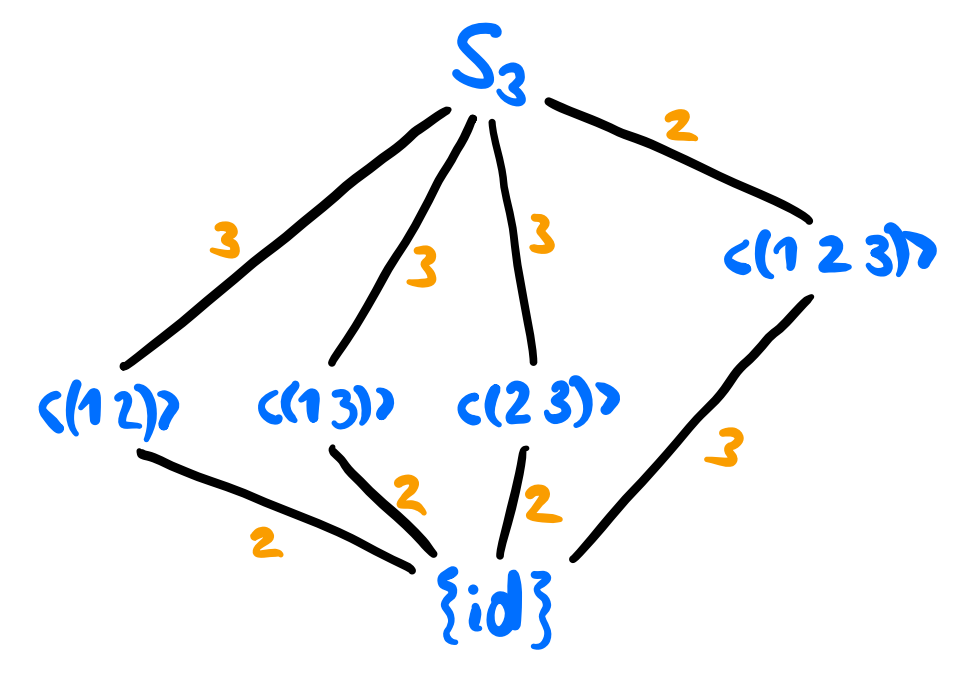
\includegraphics[width=\textwidth]{s3_subgroup_graph_index.png}
    \caption{Subgroup graph of the symmetric group $S_3$. The index of the subgroups is shown in orange.}
\end{marginfigure}

\begin{ex}{Normal subgroups (continued)}{}
\begin{itemize}
    \item $A_n \normal S_n$ as $A_n = \ker{\sgn}$, see \cref{eq:alternating_group}
    \item $\SL{n}{\R} \normal \GL{n}{\R}$ as $\SL{n}{\R} = \ker{\det}$, see \cref{eq:det_kernel}
    \item ${\Inn{G} \defeq \{i_g \mid g \in G\}}$ known as the \emph{inner automorphism group}\index{inner automorphism group} is a normal subgroup of the automorphism group, $\Inn{G} \normal \Aut{G}$
    \item For the symmetric group $S_3$, we have the normal subgroups \begin{itemize}
        \item $\{e\}, G \normal G$
        \item $A_3 = \gen{(1\ 2\ 3)} \normal G$
    \end{itemize} by \cref{lem:normal_subgroup_c}. Simple calculations confirm that the subgroups of order 2 are not normal.
\end{itemize}
\end{ex}

\begin{thm}[Quotient Group]\label{thm:quotient_group}
Let $N \normal G$. Then the set \begin{align}
    \Quot{G}{N} \defeq \{a N \mid a \in G\}
\end{align} is a group under the operation, \begin{align}
    a N \cdot b N \defeq (a \cdot b) N \quad \forall a, b \in G. \label{eq:quotient_group_op}
\end{align} $\Quot{G}{N}$ is called the \emph{quotient group}\index{quotient group} $G$ modulo $N$.
\end{thm} Thus, the quotient group is the group of (left) cosets of a normal subgroup. In particular, if $G$ is finite, we have, \begin{align}
    |\Quot{G}{N}| = \Index{G}{N} = \frac{|G|}{|N|},
\end{align} due to the \hyperref[defn:index]{definition of the index} and \hyperref[thm"lagrange]{Lagrange's theorem}. \begin{proof}
In proving that $\Quot{G}{N}$ is a group, we will see why we need the restriction of normal subgroups.

\begin{itemize}
    \item First, we need to show that the group operation \eqref{eq:quotient_group_op} is well-defined.\footnote{By \emph{well-defined}\index{well-defined function}, we mean that a function maps the same input to the same output.} Let us fix $a_1, a_2, b_1, b_2 \in G$ such that $a_1 N = a_2 N$ and $b_1 N = b_2 N$. We need to show $a_1 b_1 N = a_2 b_2 N$.
    
    As $N$ contains the neutral element $e$, we know $a_1 \in a_1 N$ and $a_2 \in a_2 N$. Therefore, $\exists n \in N.\ a_1 = a_2 n$ and, analogously, $\exists \Tilde{n} \in N.\ b_1 = b_2 \Tilde{n}$. We have, \begin{align*}
        a_1 b_1 = a_2 n b_2 \Tilde{n} = a_2 b_2 (\inv{b_2} n b_2 \Tilde{n}).
    \end{align*} Using that $N$ is normal, $\inv{b_2} n b_2 \in N$. Then, as $N$ is a subgroup, we also have $\inv{b_2} n b_2 \Tilde{n} \in N$. This shows that $a_1 b_1 N = a_2 b_2 N$.
    \item $e N = N$ is the neutral element.
    \item The group operation is closed under $\Quot{G}{N}$ by definition.
    \item $\inv{(a N)} = \inv{a} N$ clearly is the inverse of $a N$.
\end{itemize} $\implies \Quot{G}{N}$ is a group.
\end{proof}

\begin{ex}{Residue classes}{}
We will consider the quotient group $\Quot{\Z}{n\Z}$ of the group $(\Z,+)$ for any fixed $n \in \NZ$. We write, \begin{align}
    n\Z \defeq \gen{n} = \{n \cdot k \mid k \in \Z\}.
\end{align}

Observe that the left cosets are of the form \begin{align}
    a + n\Z = \{a + n \cdot k \mid k \in \Z\}.
\end{align} They are also called \emph{residue classes}\index{residue classes} modulo $n$.

To specify $\Quot{\Z}{n\Z}$, we are interested in finding when ${a + n\Z = b + n\Z}$ holds. We have, \begin{align}
    a + n\Z = b + n\Z \overset{\ref{lem:cosets_eq}}{\iff} a - b \in n\Z \overset{\ref{eq:left_coset}}{\iff} \divides{n}{a - b}.
\end{align} Equivalently to ${\divides{n}{a - b}}$, we say that $a$ is \emph{congruent}\index{congruent} $b$ modulo $n$ (denoted ${a \equiv b \mod n}$). For ${n > 0}$ this is equivalent to $a$ and $b$ having the same residue ${r \in \{0, 1, \dots, n - 1\}}$ when dividing by $n$.

From now on, we will assume ${n > 0}$. We denote elements by \begin{align}
    \rep{a} \defeq a + n\Z,
\end{align} where $a$ is referred to as the \emph{representative}\index{representative} of $\rep{a}$. It follows that, \begin{align}
    \Quot{\Z}{n\Z} = \{\rep{0}, \rep{1}, \dots, \rep{n-1}\}.
\end{align} By \cref{thm:quotient_group}, $\Quot{\Z}{n\Z}$ with the mapping ``$+$'' is a cyclic group of order $n$. It is often denoted by \begin{align}
    Z_n \defeq \Quot{\Z}{n\Z} = \gen{\rep{1}}.
\end{align}

As an example, consider $Z_8 = \{\rep{0}, \rep{1}, \rep{2}, \rep{3}, \rep{4}, \rep{5}, \rep{6}, \rep{7}\}$. We have, \vspace{-10pt}\begin{itemize}
    \item $\rep{2} + \rep{5} = \rep{7}$,
    \item $\rep{2} + \rep{6} = \rep{8} = \rep{0}$, and
    \item $\rep{-6} = \rep{2}$.
\end{itemize}
\end{ex}

\begin{defn}[Cokernel]
The \emph{cokernel}\index{cokernel} of a homomorphism ${\varphi : G \to H}$ is the quotient group $\Quot{H}{\im{\varphi}}$.
\end{defn}

\begin{ex}{Outer automorphism group}{}
Automorphisms that are not inner automorphisms are called \emph{outer automorphisms}\index{outer automorphism}. The \emph{outer automorphism group}\index{outer automorphism group} is the group of cosets of the inner automorphism group with respect to outer automorphisms, \begin{align}
    \Out{G} \defeq \Quot{\Aut{G}}{\Inn{G}}.
\end{align}

Let us define the homomorphism ${\sigma : G \to \Aut{G}, g \mapsto i_g}$. It can be shown that \vspace{-10pt}\begin{itemize}
    \item $\ker{\sigma} = Z(G)$,
    \item $\im{\sigma} = \Inn{G}$, and
    \item the cokernel of $\sigma$ is $\Out{G} = \Quot{\Aut{G}}{\Inn{G}}$.
\end{itemize}
\end{ex}

    % !TeX root = ../main.tex
% Add the above to each chapter to make compiling the PDF easier in some editors.

\chapter{Homomorphism and Isomorphism Theorems}
In this chapter, we will discuss tools to show that two groups are isomorphic.

\begin{thm}[Homomorphism Theorem]\index{homomorphism theorem}
Let $\varphi : G \to H$ be a group homomorphism. Then, \begin{align}
    \rep{\varphi} : \Quot{G}{\ker{\varphi}} \to \im{\varphi},\quad a \ker{\varphi} \mapsto \varphi(a)
\end{align} is an isomorphism. Especially, $\Quot{G}{\ker{\varphi}} \isom \im{\varphi}$.
\end{thm} \begin{proof}
\leavevmode\begin{itemize}
    \item We will first show that $\rep{\varphi}$ is well-defined. For any $a, b \in G$, \begin{align*}
        &a \ker{\varphi} = b \ker{\varphi} \\
        \iff\quad &\inv{a} b \in \ker{\varphi} \margintag{by \cref{lem:cosets_eq}} \\
        \iff\quad &\varphi(\inv{a} b) = e_H \margintag{using the definition of the kernel \eqref{eq:kernel}} \\
        \iff\quad &\inv{\varphi(a)} \varphi(b) = e_H \margintag{using that $\varphi$ is a homomorphism \eqref{eq:homomorphism}} \\
        \iff\quad &\varphi(a) = \varphi(b) \\
        \iff\quad &\rep{\varphi}(a \ker{\varphi}) = \rep{\varphi}(b \ker{\varphi}). \margintag{using the definition of $\rep{\varphi}$}
    \end{align*} The direction ``$\Rightarrow$'' shows that $\rep{\varphi}$ is well-defined. Note that ``$\Leftarrow$'' shows that $\rep{\varphi}$ is injective.
    
    \item Next, we show that $\rep{\varphi}$ is a homomorphism. For any $a, b \in G$, \begin{align*}
        \rep{\varphi}(a \ker{\varphi} \cdot b \ker{\varphi}) &= \rep{\varphi}(a b \ker{\varphi}) \margintag{using the operation of the quotient group \eqref{eq:quotient_group_op}} \\[5pt]
        &= \varphi(a b) \margintag{using the definition of $\rep{\varphi}$} \\
        &= \varphi(a) \cdot \varphi(b) \margintag{using that $\varphi$ is a homomorphism \eqref{eq:homomorphism}} \\
        &= \rep{\varphi}(a \ker{\varphi}) \cdot \rep{\varphi}(b \ker{\varphi}). \margintag{using the definition of $\rep{\varphi}$}
    \end{align*}
    
    \item Finally, we observe that $\rep{\varphi}$ is surjective. That is, for any $a \in \im{\varphi}$, we have that $a \ker{\varphi} \in \Quot{G}{\ker{\varphi}}$. \qedhere
\end{itemize}
\end{proof}

\begin{ex}{Homomorphism theorem}{}
We have already seen in \cref{ex:homomorphisms} that for any field $K$, ${\det : \GL{n}{K} \to \woZ{K}}$ is a homomorphism with ${\ker{\det} = \SL{n}{K}}$. Thus, by the homomorphism theorem, \begin{align}
    \Quot{\GL{n}{K}}{\SL{n}{K}} \isom \woZ{K}.
\end{align}
\end{ex}

\begin{marginfigure}
    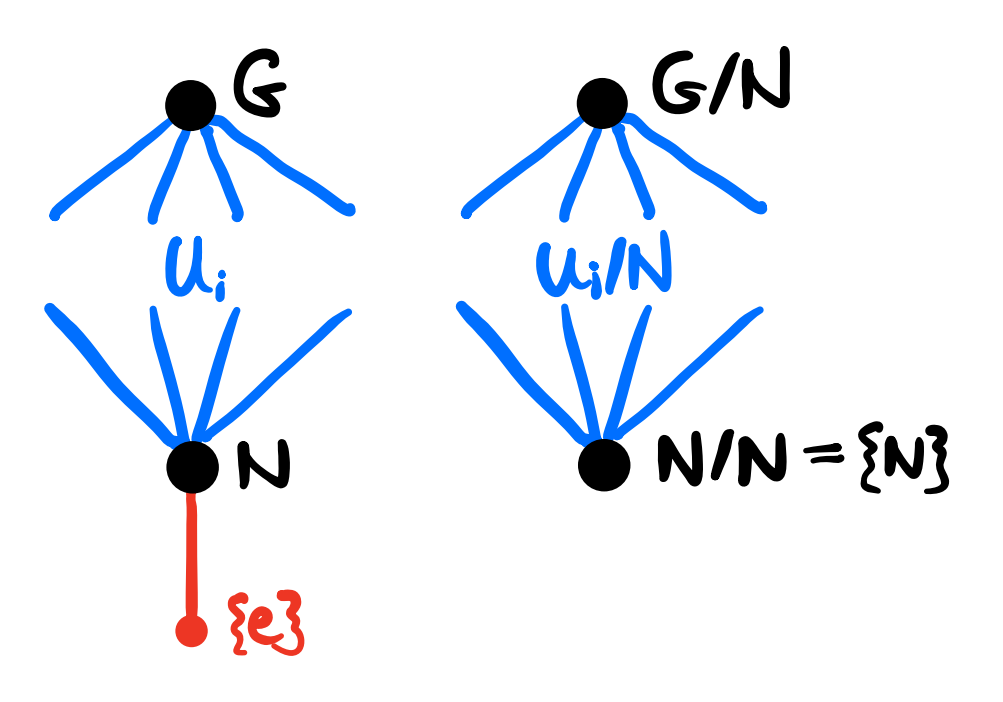
\includegraphics[width=\textwidth]{correspondence_thm.png}
    \caption{Sketch of the correspondence of subgroups $U_i$ ``between'' $G$ and $N$ and the subgroups $\Quot{U_i}{N}$ ``between'' $\Quot{G}{N}$ and $\Quot{N}{N}$.}\label{fig:correspondence_thm}
\end{marginfigure}

\begin{thm}[Correspondence Theorem]\index{correspondence theorem}
The mapping, \begin{align}
    f : \{U \subgroup G \mid N \subseteq U\} \to \{V \subgroup \Quot{G}{N}\},\quad U \mapsto \Quot{U}{N},
\end{align} is an inclusion-preserving\footnote{We say that a mapping ${f : A \to B}$ is \emph{inclusion-preserving}\index{inclusion-preserving mapping} if for any $a_1, a_2 \in A$ such that ${a_1 \subseteq a_2}$, we have ${f(a_1) \subseteq f(a_2)}$.} bijection and fore every $U \subgroup G$, \begin{align}
    U \normal G \iff \Quot{U}{N} \normal \Quot{G}{N}.
\end{align}
\end{thm} \noindent A sketch of the correspondence theorem is given in \cref{fig:correspondence_thm}.

\begin{marginfigure}
    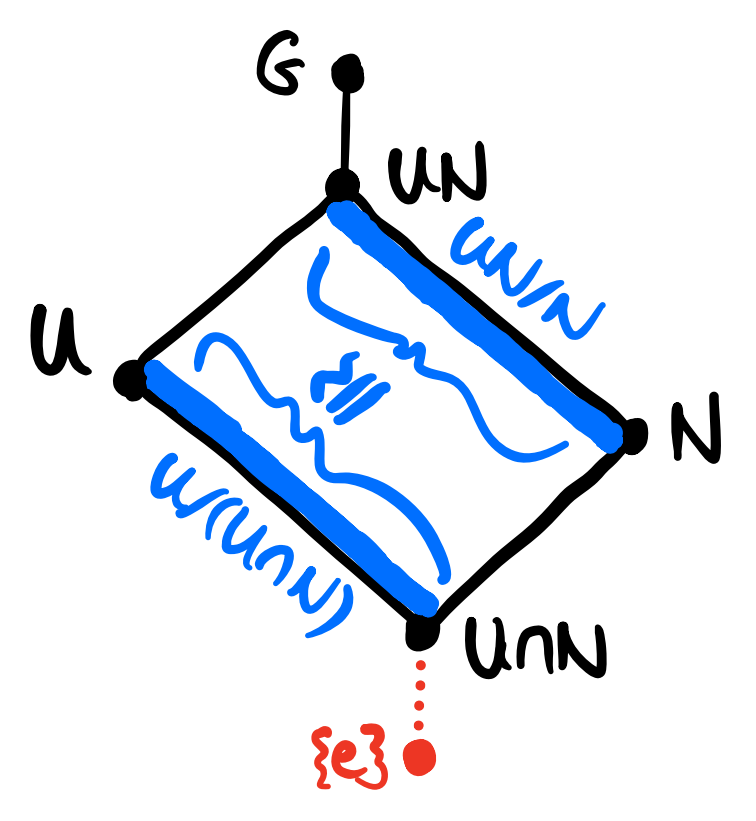
\includegraphics[width=\textwidth]{first_isom_thm.png}
    \caption{Sketch of the first isomorphism theorem.}\label{fig:first_isom_thm}
\end{marginfigure}

\begin{thm}[First Isomorphism Theorem]\index{first isomorphism theorem}\index{isomorphism theorem}
Let $U \subgroup G$ and $N \normal G$. Then, \begin{thmlist}
    \item $U N \subgroup G$ where $U N \defeq \{x \cdot n \mid x \in U, n \in N\}$
    \item $U \cap N \normal U$
    \item $\Quot{UN}{N} \isom \Quot{U}{(U \cap N)}$
\end{thmlist}
\end{thm} \noindent A sketch of the correspondence theorem is given in \cref{fig:first_isom_thm}.

\begin{marginfigure}
    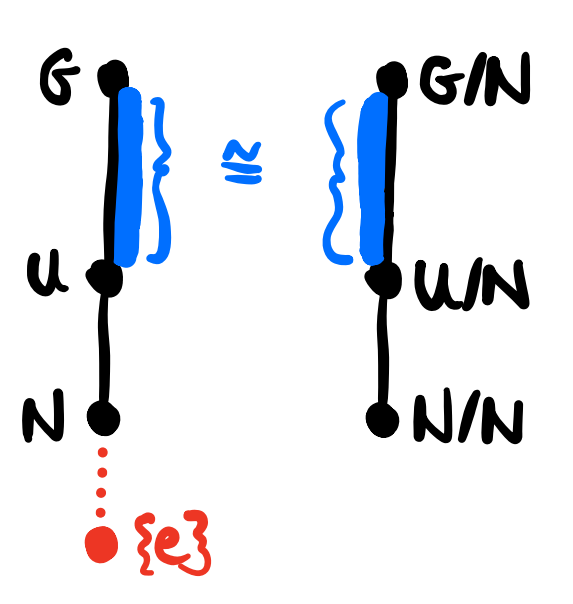
\includegraphics[width=\textwidth]{second_isom_thm.png}
    \caption{Sketch of the second isomorphism theorem..}\label{fig:second_isom_thm}
\end{marginfigure}

\begin{thm}[Second Isomorphism Theorem]\index{second isomorphism theorem}\index{isomorphism theorem}
Let $U, N \normal G$ with $N \subseteq U$. Then, $\Quot{(\Quot{G}{N})}{(\Quot{U}{N})} \isom \Quot{G}{U}$.
\end{thm}
    % !TeX root = ../main.tex
% Add the above to each chapter to make compiling the PDF easier in some editors.

\chapter{Group Actions}\label{sec:groups:actions}
    % !TeX root = ../main.tex
% Add the above to each chapter to make compiling the PDF easier in some editors.

\chapter{Sylow Theorems}
    % !TeX root = ../main.tex
% Add the above to each chapter to make compiling the PDF easier in some editors.

\chapter{Direct Products and Abelian Groups}
    % !TeX root = ../main.tex
% Add the above to each chapter to make compiling the PDF easier in some editors.

\chapter{Solvable Groups}
    
    \part{Rings}\label{cha:rings}
    % !TeX root = ../main.tex
% Add the above to each chapter to make compiling the PDF easier in some editors.

\chapter{Rings and Ideals}
    % !TeX root = ../main.tex
% Add the above to each chapter to make compiling the PDF easier in some editors.

\chapter{Homomorphisms and Quotient Rings}
    % !TeX root = ../main.tex
% Add the above to each chapter to make compiling the PDF easier in some editors.

\chapter{Divisors in Integral Domains}
    % !TeX root = ../main.tex
% Add the above to each chapter to make compiling the PDF easier in some editors.

\chapter{Polynomial Rings}
    % !TeX root = ../main.tex
% Add the above to each chapter to make compiling the PDF easier in some editors.

\chapter{Factorial Rings}
    % !TeX root = ../main.tex
% Add the above to each chapter to make compiling the PDF easier in some editors.

\chapter{Euclidean Domains and Principal Ideal Domains}
    % !TeX root = ../main.tex
% Add the above to each chapter to make compiling the PDF easier in some editors.

\chapter{Irreducibility of Polynomials}
    
    \part{Fields}\label{cha:fields}
    % !TeX root = ../main.tex
% Add the above to each chapter to make compiling the PDF easier in some editors.

\chapter{Fields}
\begin{defn}[Field]\label{defn:field}
\end{defn}
    % !TeX root = ../main.tex
% Add the above to each chapter to make compiling the PDF easier in some editors.

\chapter{Algebraic Field Extensions}
    % !TeX root = ../main.tex
% Add the above to each chapter to make compiling the PDF easier in some editors.

\chapter{Splitting Fields}
    % !TeX root = ../main.tex
% Add the above to each chapter to make compiling the PDF easier in some editors.

\chapter{Normal and Separable Field Extensions}
    % !TeX root = ../main.tex
% Add the above to each chapter to make compiling the PDF easier in some editors.

\chapter{Galois Theory}
    % !TeX root = ../main.tex
% Add the above to each chapter to make compiling the PDF easier in some editors.

\chapter{Finite Fields}
    % !TeX root = ../main.tex
% Add the above to each chapter to make compiling the PDF easier in some editors.

\chapter{Cyclotomic Fields}
    % !TeX root = ../main.tex
% Add the above to each chapter to make compiling the PDF easier in some editors.

\chapter{Solvable Polynomials}

    \backmatter

    % !TeX root = ../main.tex
% Add the above to each chapter to make compiling the PDF easier in some editors.

\chapter{Summary of Notation}

\begin{fullwidth}
We follow these general rules: \begin{itemize}[noitemsep]
    % \item uppercase italic for constants $N$
    \item lowercase italic for indices $i$ and scalar variables $a$
    % \item lowercase italic bold for vectors $\vx$
    \item uppercase italic bold for matrices $\mM$
    % \item uppercase italic for random variables $X$
    % \item uppercase bold for random vectors $\rX$
    \item uppercase italic for sets $A$
    % \item uppercase calligraphy for spaces (usually infinite sets) $\spA$
\end{itemize}

\emptyparagraph\begin{tabular}{p{2cm}l}
    $\defeq$ & equality by definition \\
    $f : A \to : B$ & function $f$ from elements of set $A$ to elements of set $B$ \\
    $\N$ & set of natural numbers $\{1, 2, \dots\}$ \\
    $\NZ$ & set of natural numbers, including $0$, $\N \cup \{0\}$ \\
    $[n]$ & set of natural numbers from $1$ to $n$, $\{1, 2, \dots, n-1, n\}$ \\
    $\Z$ & set of integers $\{\dots, -2, 1, 0, 1, 2, \dots\}$ \\
    $\R$ & set of real numbers \\
    $\C = \R^2$ & set of complex numbers \\
\end{tabular}

\section*{\smallcaps{Groups}}
\emptyparagraph\begin{tabular}{p{2cm}l}
    $\GL{n}{K}$ & \emph{general linear group} over invertible linear maps $\mA \in K^{n \times n}$, $\determ{\mA} \neq 0$ \\
    $\SL{n}{K}$ & \emph{special linear group} over volume-preserving linear maps $\mA \in K^{n \times n}$, $\determ{\mA} = 1$ \\
    $S_n$ & \emph{symmetric group} over bijections on $[n]$ (so-called permutations) \\
\end{tabular}
\end{fullwidth}


    % \nocite{*}
    % \bibliography{sources}

    \begin{fullwidth}
    \printindex
    \end{fullwidth}
\end{document}
